% =====================================================================
% schema_newton_l1.tex — Schema Newton-CG L1, fig:newton_l1 della tesi
% Stesso codice TikZ della tesi; compilare con pdflatex.
% =====================================================================
\documentclass[border=8pt]{standalone}
\usepackage[T1]{fontenc}
\usepackage[utf8]{inputenc}
\usepackage{amsmath, amssymb}
\usepackage{tikz}
\usetikzlibrary{arrows.meta, positioning, calc}
\definecolor{coverblue}{RGB}{30, 60, 120}

\begin{document}
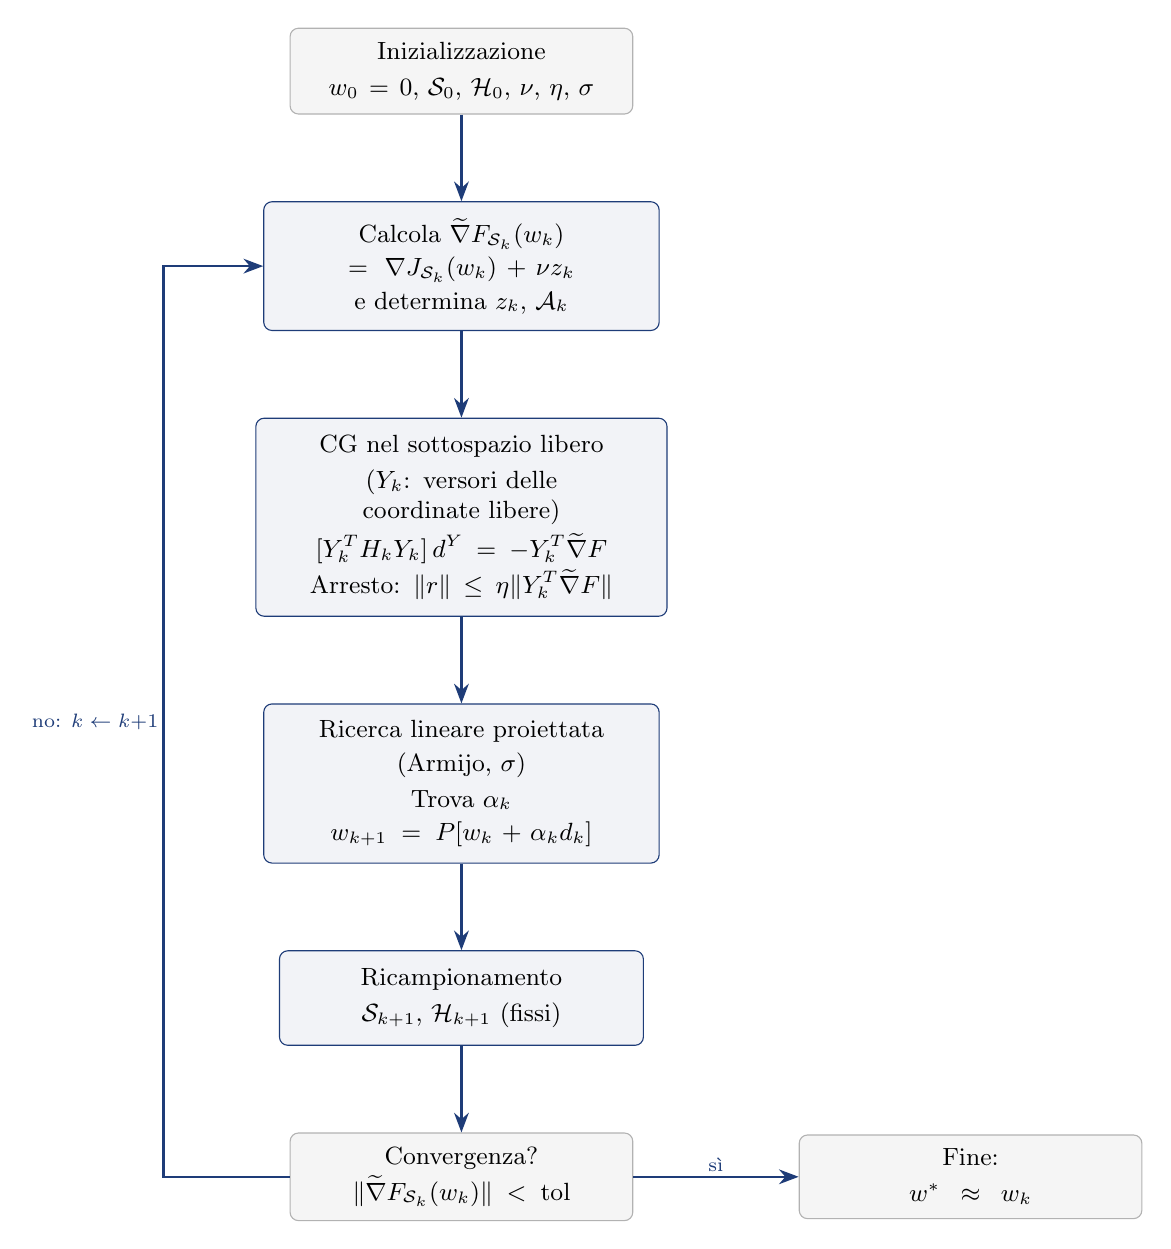
\begin{tikzpicture}[
  node distance=1.1cm and 2.4cm,
  every node/.style={font=\small},
  box/.style={
    draw=coverblue, fill=coverblue!6, rounded corners=3pt,
    text width=4.2cm, align=center, minimum height=1.2cm,
    inner sep=6pt
  },
  io/.style={
    draw=gray!60, fill=gray!8, rounded corners=3pt,
    text width=4.0cm, align=center, minimum height=1.0cm,
    inner sep=5pt
  },
  arrow/.style={-{Stealth[length=2.5mm]}, thick, color=coverblue},
  label/.style={font=\scriptsize, fill=white, inner sep=1.5pt}
]

  % Nodi principali (colonna centrale)
  \node[io] (init) {Inizializzazione\\[2pt] $w_0=0$, $\mathcal{S}_0$, $\mathcal{H}_0$, $\nu$, $\eta$, $\sigma$};
  \node[box, below=of init, text width=4.6cm, minimum height=1.4cm] (subgrad) {Calcola $\widetilde{\nabla}F_{\mathcal{S}_k}(w_k)$\\[1pt] $=\nabla J_{\mathcal{S}_k}(w_k)+\nu z_k$\\[1pt] e determina $z_k$, $\mathcal{A}_k$};
  \node[box, below=of subgrad, text width=4.8cm, minimum height=1.6cm] (cg) {CG nel sottospazio libero\\[2pt] ($Y_k$: versori delle coordinate libere)\\[2pt] $[Y_k^T H_k Y_k]\,d^Y = -Y_k^T \widetilde{\nabla}F$\\[1pt] Arresto: $\|r\| \le \eta\|Y_k^T \widetilde{\nabla}F\|$};
  \node[box, below=of cg, text width=4.6cm, minimum height=1.4cm] (ls) {Ricerca lineare proiettata\\[1pt] (Armijo, $\sigma$)\\[2pt] Trova $\alpha_k$\\[1pt] $w_{k+1} = P[w_k + \alpha_k d_k]$};
  \node[box, below=of ls] (recamp) {Ricampionamento\\[2pt] $\mathcal{S}_{k+1}$, $\mathcal{H}_{k+1}$ (fissi)};
  \node[io, below=of recamp] (conv) {Convergenza?\\[2pt] $\|\widetilde{\nabla}F_{\mathcal{S}_k}(w_k)\| < \mathrm{tol}$};
  \node[io, right=2.1cm of conv] (end) {Fine:\\[2pt] $w^* \approx w_k$};

  % Frecce verticali principali
  \draw[arrow] (init) -- (subgrad);
  \draw[arrow] (subgrad) -- (cg);
  \draw[arrow] (cg) -- (ls);
  \draw[arrow] (ls) -- (recamp);
  \draw[arrow] (recamp) -- (conv);

  % Freccia uscita
  \draw[arrow] (conv) -- (end) node[label, midway, above] {sì};

  % Loop ritorno da conv a subgrad (percorso esterno sinistro)
  \draw[arrow] (conv.west) -- ++(-1.6,0) |- (subgrad.west)
    node[label, pos=0.25, left] {no: $k \leftarrow k{+}1$};

\end{tikzpicture}
\end{document}
